\documentclass[a4paper]{article}
\usepackage{geometry}
\usepackage[utf8]{inputenc}
\usepackage[T1]{fontenc}
\usepackage[bookmarks,colorlinks]{hyperref}
\usepackage[french]{babel}
\usepackage{pdflscape}
\usepackage{graphicx}

\title{Rapport d'analyse du projet de Technologies Objets}
\author{Maxime Arthaud \and Korantin Auguste \and Martin Carton}
\date{24 Mai 2013}

\begin{document}
\maketitle

\section{Scénarios d'utilisation}
  Génération d'image à partir d'une scène 3D comportant des objets simples.

\section{Démarche}
  Nous avons commencé par faire la liste des choses à faire. Nous avons décidé
  de séparer l'interface graphique de la partie génération d'image. L'interface
  graphique permettra de générer un fichier contenant toutes les informations
  nécessaires à la génération de l'image qui sera faite par un second programme
  utilisable en ligne de commande, ce fichier sera simple et pourra être écrit
  à la main.

\section{Tâches effectuées}
  Nous avons commencé à réfléchir à l'organisation des classes, à l'interface
  utilisateur et au format de fichier.

  \subsection{Diagramme d'analyse}
    La figure \ref{fig:uml} présente les relations entre les différentes classes
    que nous envisageons d'utiliser.

  \subsection{Interface utilisateur}
    La figure \ref{fig:gui} présente l'interface graphique telle que nous
    envisageons de la faire.

    Les différents objets (caméra (c'est à dire point de vue et écran),
    sphères, cubes et plans) peuvent être y ajoutés selon leurs différentes
    propriétés optiques et supprimés. Un résumé des objets créés est affiché, on
    peut directement lancer la génération de l'image, ou enregistrer le fichier.

  %\subsection{Diagramme de séquence}
  \subsection{Format de fichier}
    Le fichier sera un fichier texte où chaque objet sera représenté sur une
    ligne. Chaque ligne sera de la forme
    \verb+Nom(nom1=valeur1, nom2=valeur2, .., nomN=valeurN)+ où \verb+Nom+ est
    le nom de l'objet à créer (Camera, Sphere, Cube ou Plane), et les noms et
    valeurs sont les données qui caractérisent l'objet, par exemple le rayon
    et le centre pour la Sphere, ou encore la réflectance.

    \newgeometry{width=1.3\linewidth}
    \begin{landscape}
      \thispagestyle{empty}
      \begin{figure}[p]
        \makebox[\paperwidth][c]{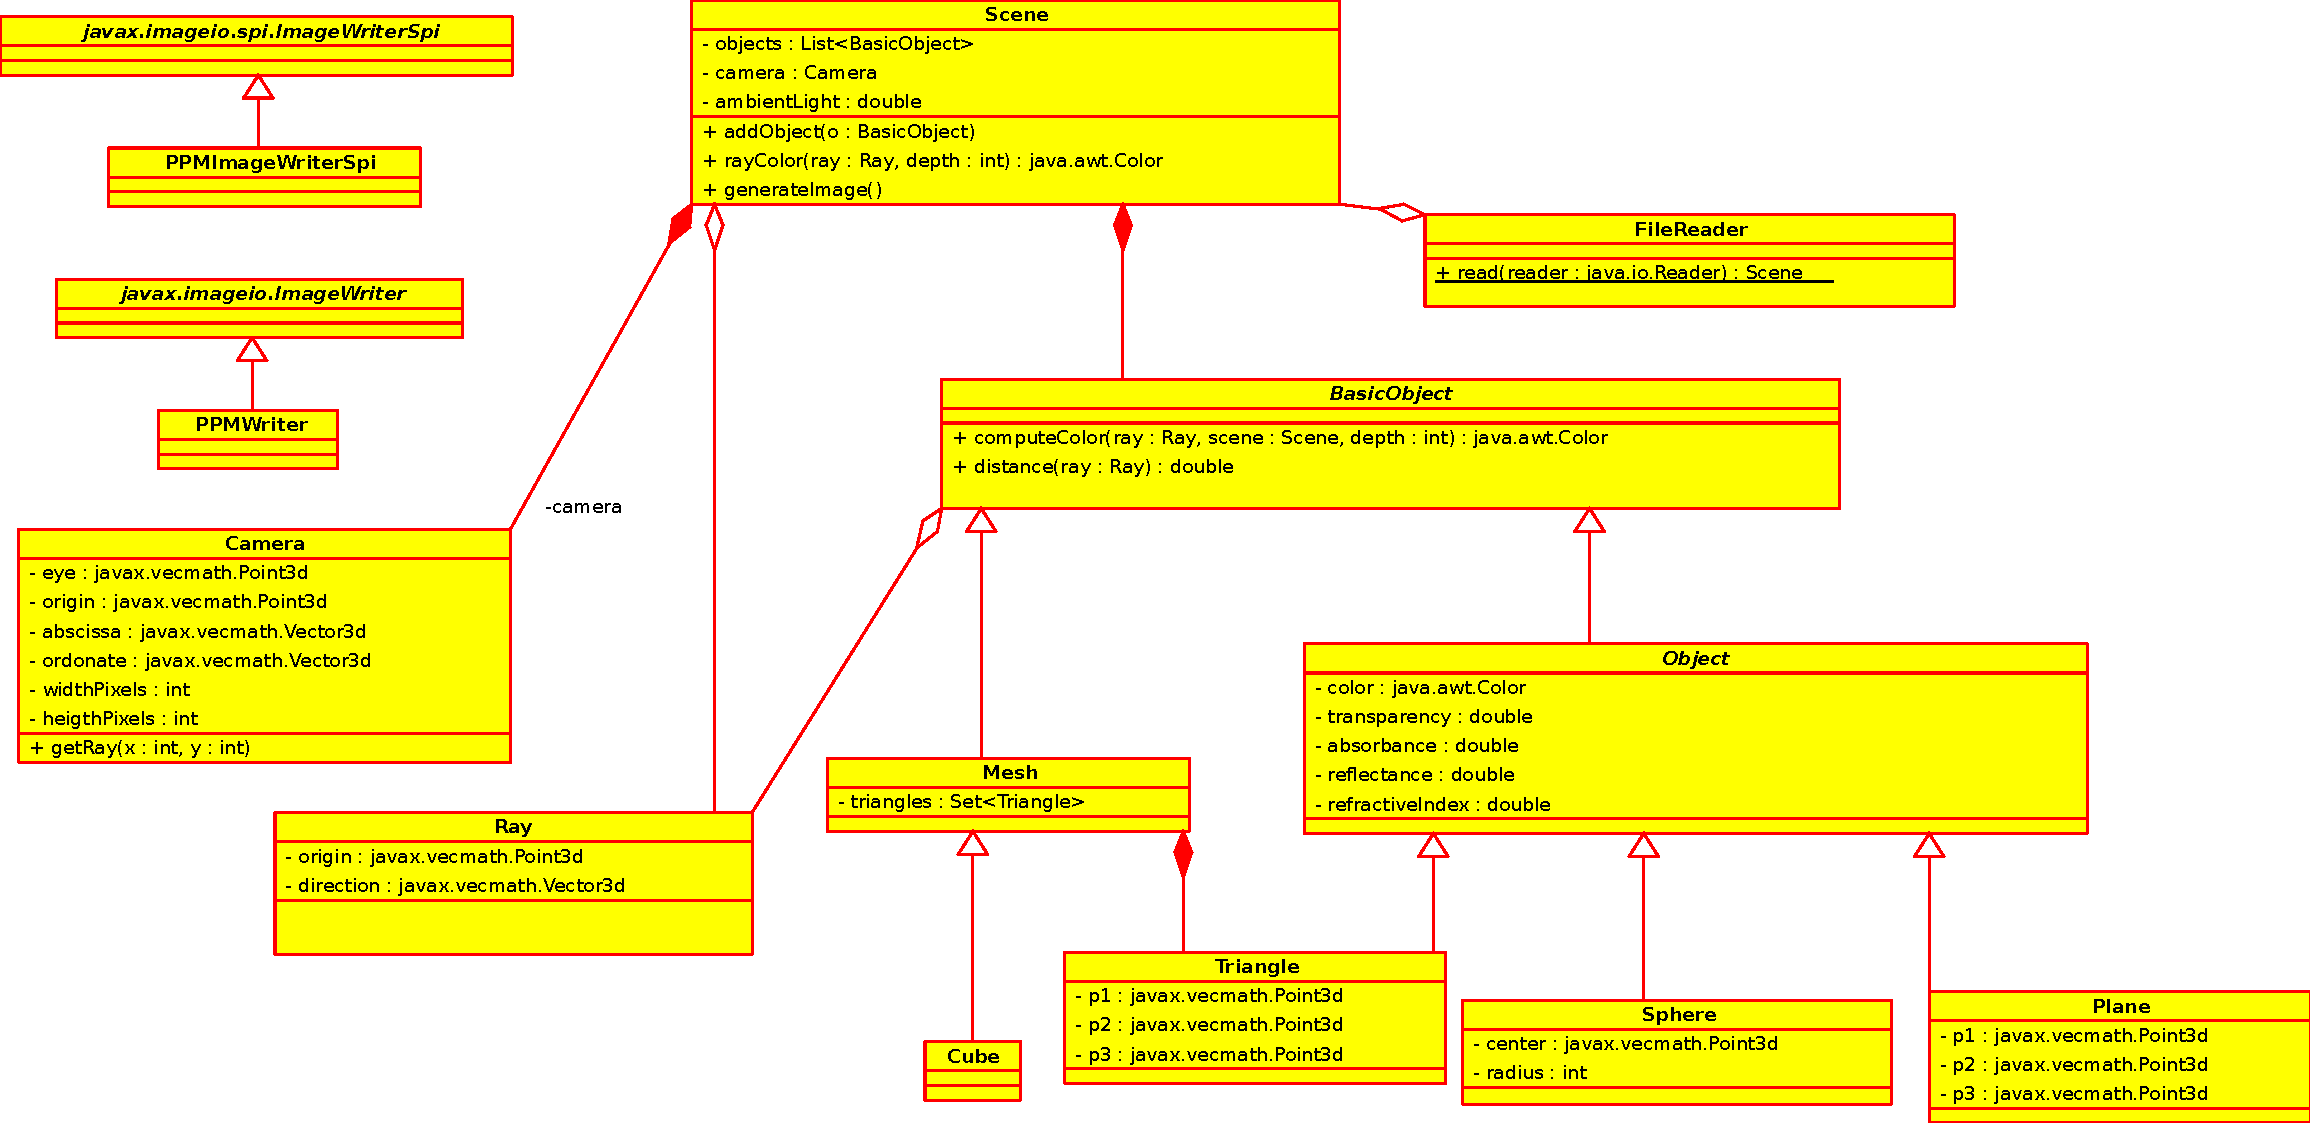
\includegraphics[width=26cm]{uml.pdf}}
        \caption{Diagramme UML\label{fig:uml}}
      \end{figure}
    \end{landscape}
    \restoregeometry

    \begin{figure}[p]
      \centerline{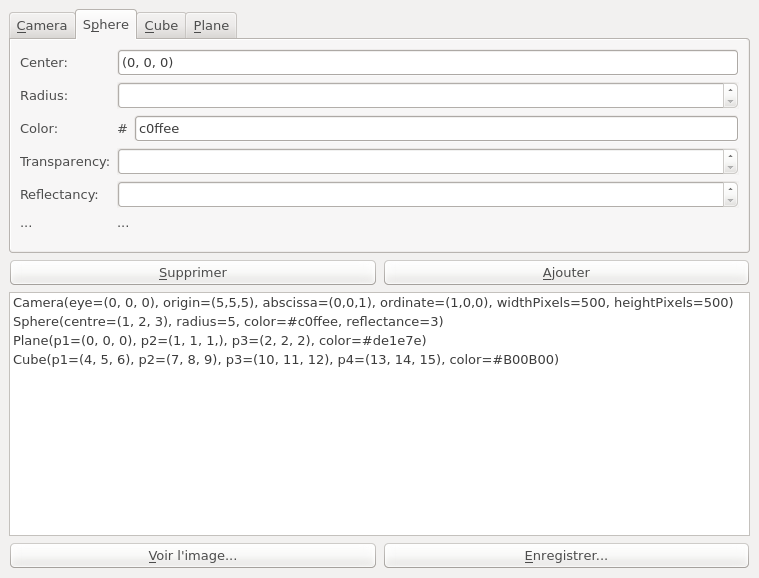
\includegraphics[width=1.2\textwidth]{gui.png}}
    \caption{Interface graphique\label{fig:gui}}
    \end{figure}

\end{document}

